%! TEX root = ../main.tex
% ==============================================================
% IMMUTABLE — generated automatically, do not edit this block
%
% — Provenance ───────────────────────────────────────────────────
%   script            : plotter.py
%   computed_in       : plotter.py::plot_probe_noise_floor (per-run Amplitude / Stillwater Std from combined_meta)
%   plot_type         : probe_noise_floor
%   data_class        : DFS
%   generated_at      : 2026-05-05T13:12:44
%   findings_doc      : 
%
% — Thesis context ──────────────────────────────────────────────
%   chapter           : 04
%   caption_label     : fig:ch04_probe_noise_floor
%   caption_short     : Probes støygulv
%
% — Filters ────────────────────────────────────────────────────
%   panel             : 
%   wind              : 
%   amplitude [V]     : 
%   frequency [Hz]    : 
%   probes            : 
%   run_category      : nowave_control
%   quality_flag      : 
%   mooring           : 
%
% — Data provenance ────────────────────────────────────────────
%   n_runs            : 609
%   in_probes_used    : 9373/170+9373/340, 9373/250
%   out_probes_used   : 11800/250, 12400/170+12400/340, 12400/250
%   probe_configs     : initial_setup, march2026_better_rearranging, march2026_rearranging, nov_normalt_oppsett
%   non_final_config_n: 141
%   datasets        :
%     PROCESSED-20260326-ProbePos4_31_FPV_2-tett6roof-under9Mooring-height100-lowrange
%     PROCESSED-20260327-ProbePos4_31_FPV_2-tett6roof-under9Mooring30-height100-lowrange
%   run_paths       :
%     (omitted — aggregate over > threshold runs, see datasets)
%
% — Method / numerical parameters ─────────────────────────────
%   grouper           : stillwater aggregation (group_by=probe_height_mm,probe_range_mode)
%   collapse_panels   : False
%   fft_window_hz     : 0.1
%   extra_params      : k_sigma=3.0, k_q=2.0, highlight_keyword=None, exclude_keywords=['nestenstille'], threshold=max(k_sigma·σ, k_q·q)
%
% — Method documentation ────────────────────────────────────
%   Per-probe metrics — one row per (group, probe) in `summary`:
%
%     σ      = `Probe {pos} Stillwater Std` — sample std-dev of
%              the raw stillwater signal during the run [mm].
%     amp99  = `Probe {pos} Amplitude` — half the central 99 %
%              range: (P99.5 − P0.5) / 2 [mm]. Robust to non-
%              Gaussian tails. Note: column name uses legacy
%              '95pct' suffix; the value is the 99 % half-range.
%     q      = quantization step — P5 of nonzero |Δη| between
%              consecutive samples in eta_{pos}_interp [mm].
%              Smallest non-zero output the probe ever reports.
%              NaN when processed_dfs is not loaded at the time
%              the cell runs (light tier in main_save_figures).
%
%   Group aggregation (mean over accepted stillwater runs):
%     noise_rms_mm          = mean(σ)
%     noise_99pct_amp_mm    = mean(amp99)            ← bar height
%     noise_99pct_std_mm    = std(amp99)             ← errorbar
%     quantization_step_mm  = q (first run with data)
%     bias_vs_ref_mm        = mean(level) − cross-probe mean,
%                             where level = `Stillwater Probe {pos}`.
%
%   Detection threshold (red dashed line per probe):
%     threshold_mm = max(k_sigma · noise_rms_mm,
%                        k_q     · quantization_step_mm)
%                  = max(3·σ̄, 2·q).
%     A signal below this line cannot be reliably distinguished
%     from probe random noise (k_sigma·σ ≈ 99.7 % CI for Gaussian)
%     AND probe quantization (k_q·q = k_q output-grid steps).
%     The dotted grey line shows q/2.
%
%   Run filtering (visible only in the figure, not in stats):
%     exclude_keywords    : ['nestenstille'] → dropped from
%                           the aggregation entirely (treated as
%                           not-settled).
%     highlight_keyword   : None → marked with a
%                           gold star, included in stats.
%     show_excluded       : when False (caller's choice), the X
%                           markers + legend entry for excluded
%                           runs are hidden; runs are still
%                           excluded from aggregation.
%
% — Summary stats cited in caption ────────────────────────────
%   stat:n_groups     : 4
%   stat:n_probes     : 4
%   stat:k_sigma      : 3.0
%   stat:k_q          : 2.0
%   stat:noise_mm_9373/170 : 0.146
%   stat:threshold_mm_9373/170 : 0.23
%   stat:noise_mm_12400/250 : 0.132
%   stat:threshold_mm_12400/250 : 0.191
%   stat:noise_mm_9373/340 : 0.098
%   stat:threshold_mm_9373/340 : 0.163
%   stat:noise_mm_8804/250 : 0.135
%   stat:threshold_mm_8804/250 : 0.182
%
% — Subfigures available ───────────────────────────────────────
%     FIGURES/ch04_probe_noise_floor_group0.pdf
%     FIGURES/ch04_probe_noise_floor_group1.pdf
%     FIGURES/ch04_probe_noise_floor_group2.pdf
%     FIGURES/ch04_probe_noise_floor_group3.pdf
% ── end immutable block ─────────────────────────────────────────
\begin{figure}[htbp]
  \centering
  \begin{subfigure}[b]{0.48\linewidth}
    \centering
    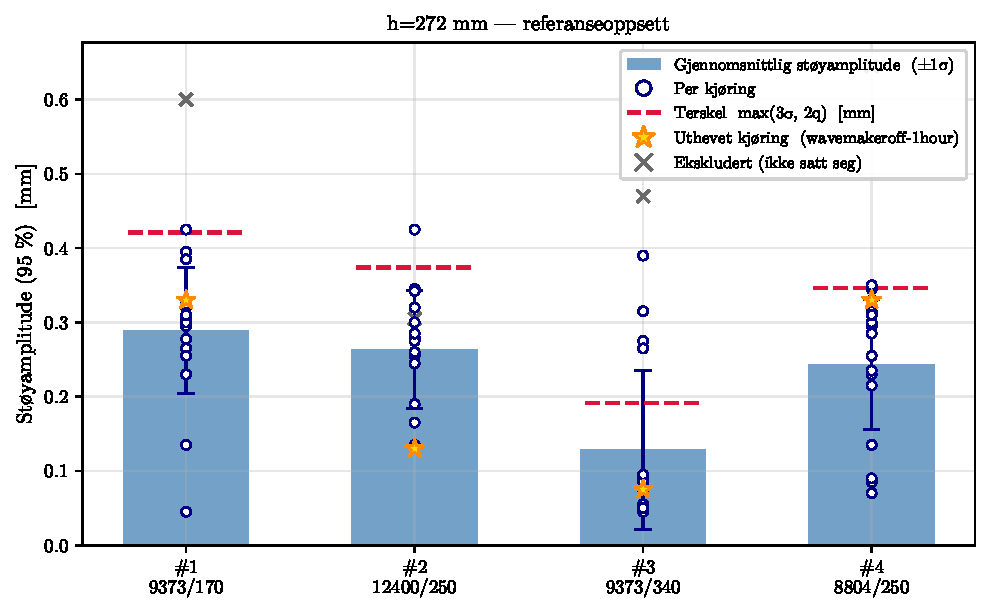
\includegraphics[width=\linewidth]{FIGURES/ch04_probe_noise_floor_group0.pdf}
    \caption{Prober hengende høyt over vannet.}
    \label{fig:ch04_probe_noise_floor_group0}
  \end{subfigure}
  \hfill
  \begin{subfigure}[b]{0.48\linewidth}
    \centering
    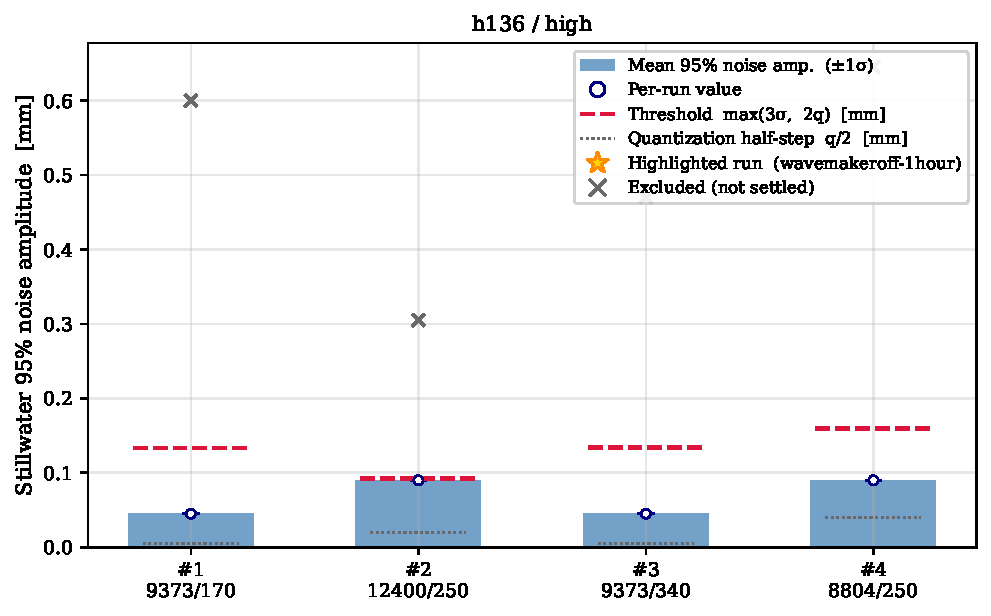
\includegraphics[width=\linewidth]{FIGURES/ch04_probe_noise_floor_group1.pdf}
    \caption{TODO}
    \label{fig:ch04_probe_noise_floor_group1}
  \end{subfigure}
  \hfill
  \begin{subfigure}[b]{0.48\linewidth}
    \centering
    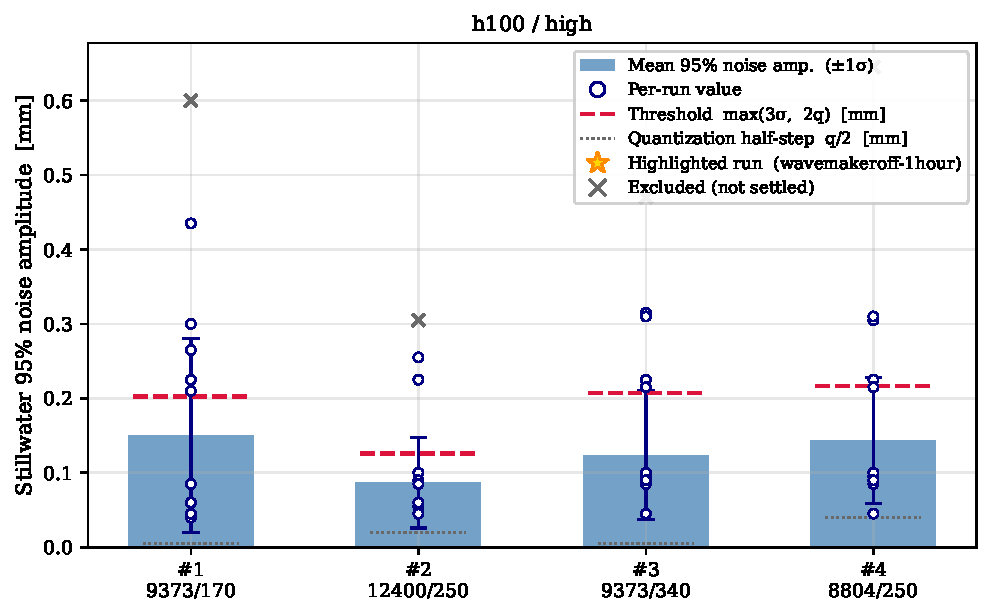
\includegraphics[width=\linewidth]{FIGURES/ch04_probe_noise_floor_group2.pdf}
    \caption{TODO}
    \label{fig:ch04_probe_noise_floor_group2}
  \end{subfigure}
  \hfill
  \begin{subfigure}[b]{0.48\linewidth}
    \centering
    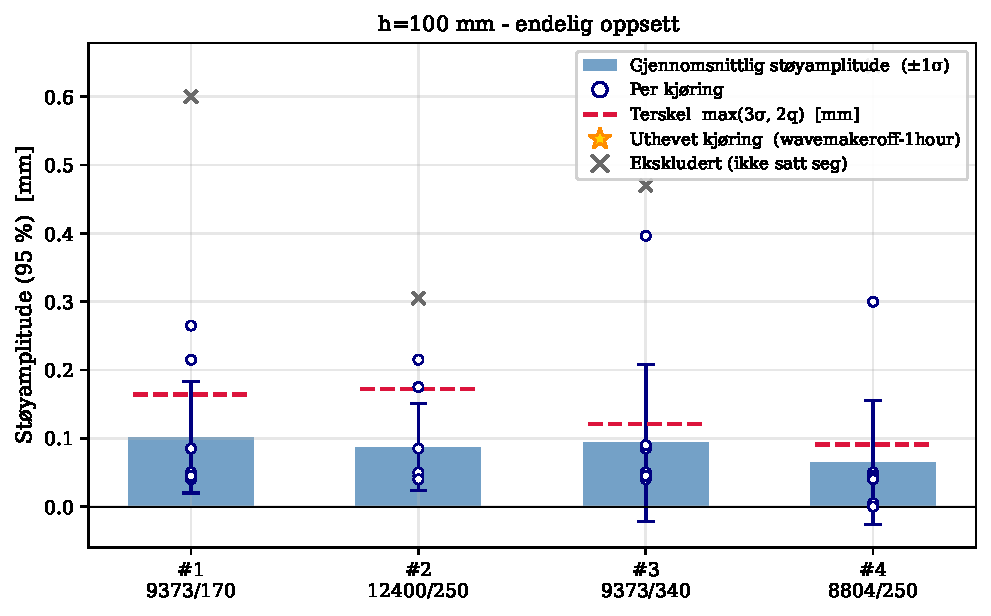
\includegraphics[width=\linewidth]{FIGURES/ch04_probe_noise_floor_group3.pdf}
    \caption{Prober hengende lavt over vannet.}
    \label{fig:ch04_probe_noise_floor_group3}
  \end{subfigure}
  \caption[Probes støygulv]{
    Hver enkelt probes støygulv
  }
  \label{fig:ch04_probe_noise_floor}
\end{figure}
